\documentclass[12pt, xcolor=beamer,table,usenames,dvipsnames, ignorenonframetext, ngerman,t]{beamer}
\usetheme{Frankfurt}
\usecolortheme{dove}
\usepackage{appendixnumberbeamer}
%\setbeamersize{text margin left=20pt,text margin right=20pt,}

\beamertemplatenavigationsymbolsempty 
\setbeamertemplate{headline}{}
\setbeamertemplate{itemize item}{\textbullet}

\addtobeamertemplate{navigation symbols}{}{
	\ifnum\insertframenumber>\inserttotalframenumber%
	\relax
	\else%
	\usebeamerfont{footline}%
	\usebeamercolor[fg]{footline}%
	\hspace{1em}%
	\insertframenumber
	\fi%
}
\addtobeamertemplate{frametitle}{\vspace*{.2cm}}{\vspace*{.2cm}}

\setbeamercolor{footline}{fg=black}
\usepackage{soul}
\makeatletter
\let\HL\hl
\renewcommand\hl{%
	\let\set@color\beamerorig@set@color
	\let\reset@color\beamerorig@reset@color
	\HL}

\usepackage{tipa}
\usepackage{tikz}
\usetikzlibrary{shapes.geometric, arrows}
\mode<presentation>

  \setbeamercovered{invisible}
\usepackage{multicol}
\usepackage[english]{babel}
\usepackage[latin1]{inputenc}
\usepackage{times}
\usepackage[T1]{fontenc}
\usepackage{ulem}
\usepackage{tipa}
\usepackage{qtree}
\usepackage{phonrule}
\usepackage{graphicx}
\usepackage{apacite}
\usepackage{xcolor}
\setlength\parindent{0pt}
\usepackage{natbib}
\usepackage{tikz}
\usetikzlibrary{arrows.meta}
\usepackage{tcolorbox}
\tcbuselibrary{raster}

\newcommand{\bluecheck}{}%
\DeclareRobustCommand{\greencheck}{%
	\tikz\fill[scale=0.6, color=ForestGreen]
	(0,.35) -- (.25,0) -- (1,.7) -- (.25,.15) -- cycle;%
}


\begin{document}

\begin{frame}{ }
\vskip 6em

\begin{center}
{\Large Multi-party communication games}

\bigskip


{\large Veronica Boyce}

\bigskip





\end{center}
\end{frame}



\begin{frame}{Theoretical background}
	\begin{itemize}
		\item Conventionalization
		\item Conversation of two people
		\item Reference 
		\item Also want to connect this to teaching 
	\end{itemize}
\end{frame}


%
\begin{frame}{Clark \& Wilkes-Gibbs 1986}
	
	\begin{itemize}
		\item How do people coordinate in a conversation? 
		%People don't cleanly take turns, don't use full utterances, can do lots of confirmation or repair. 
		\item How do people refer? 
		% counter to idealized linguistic or philosophical models, it's messy
		\item Idea that there's some sort of "acceptance" of reference
	%	\item Tangram reference game has earlier antecedents, but this is foundational to reference coordination, conversational pacts
	%	\item Originates using *this* set of tangrams
		%\item Ordering task, 12 tangrams x 6 rounds, oral communication
	%	\item Timed and transcribed
		\item 8 dyads 
	%	\item Number of words declines over trials steeply between 1 \& 2 and then asymptotes
	%	\item Number of turns also declines
	%	\item Referents become more definite, less hedged
	%	\item Lots of qualitative descriptions
	\end{itemize}
	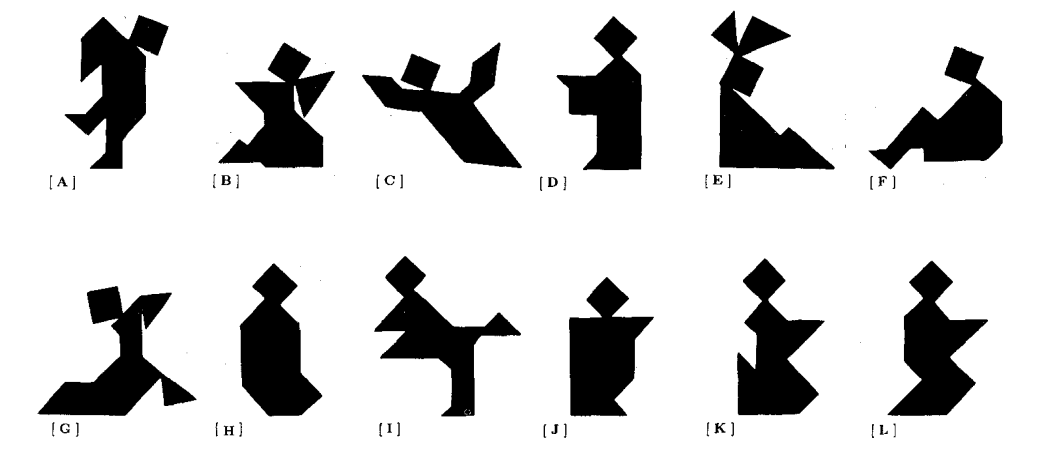
\includegraphics[width=\textwidth]{images/clark_tangrams.png}
\end{frame}

\begin{frame}{Clark \& Wilkes-Gibbs 1986}
	
	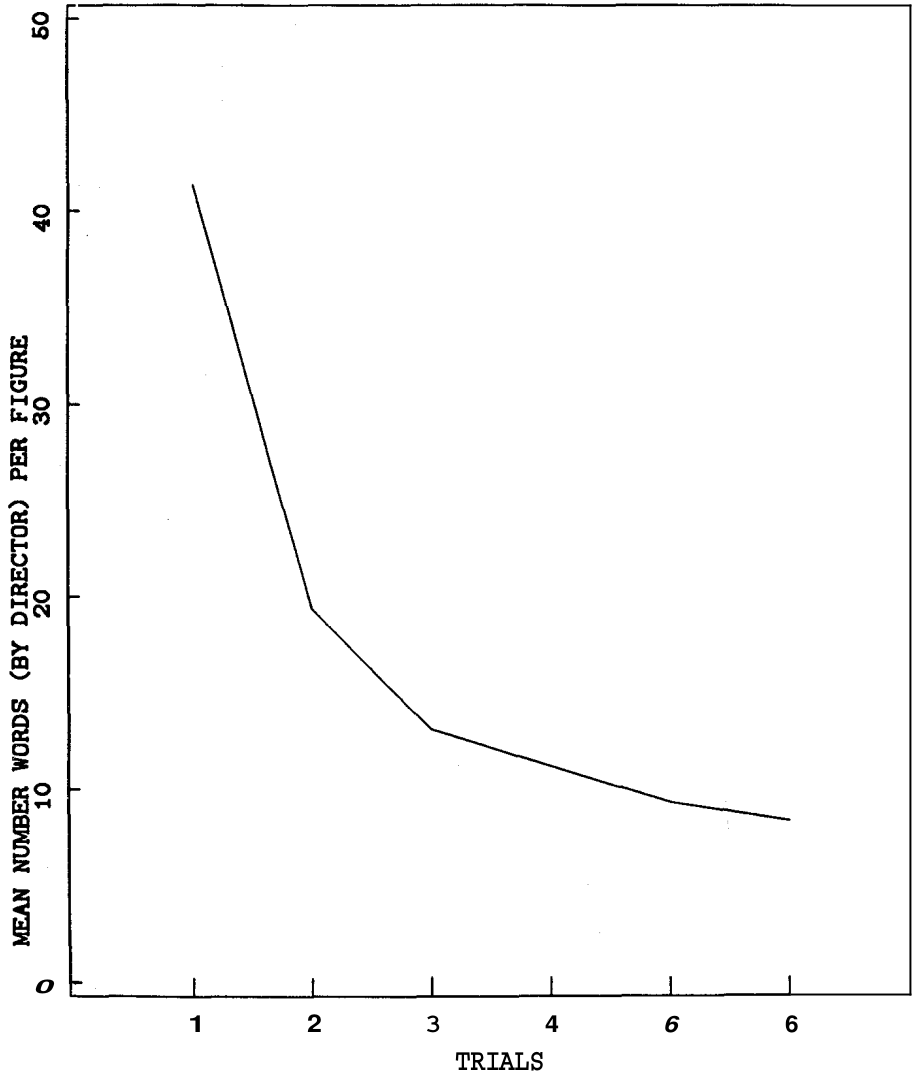
\includegraphics[width=.48\textwidth]{images/clark_words.png}
		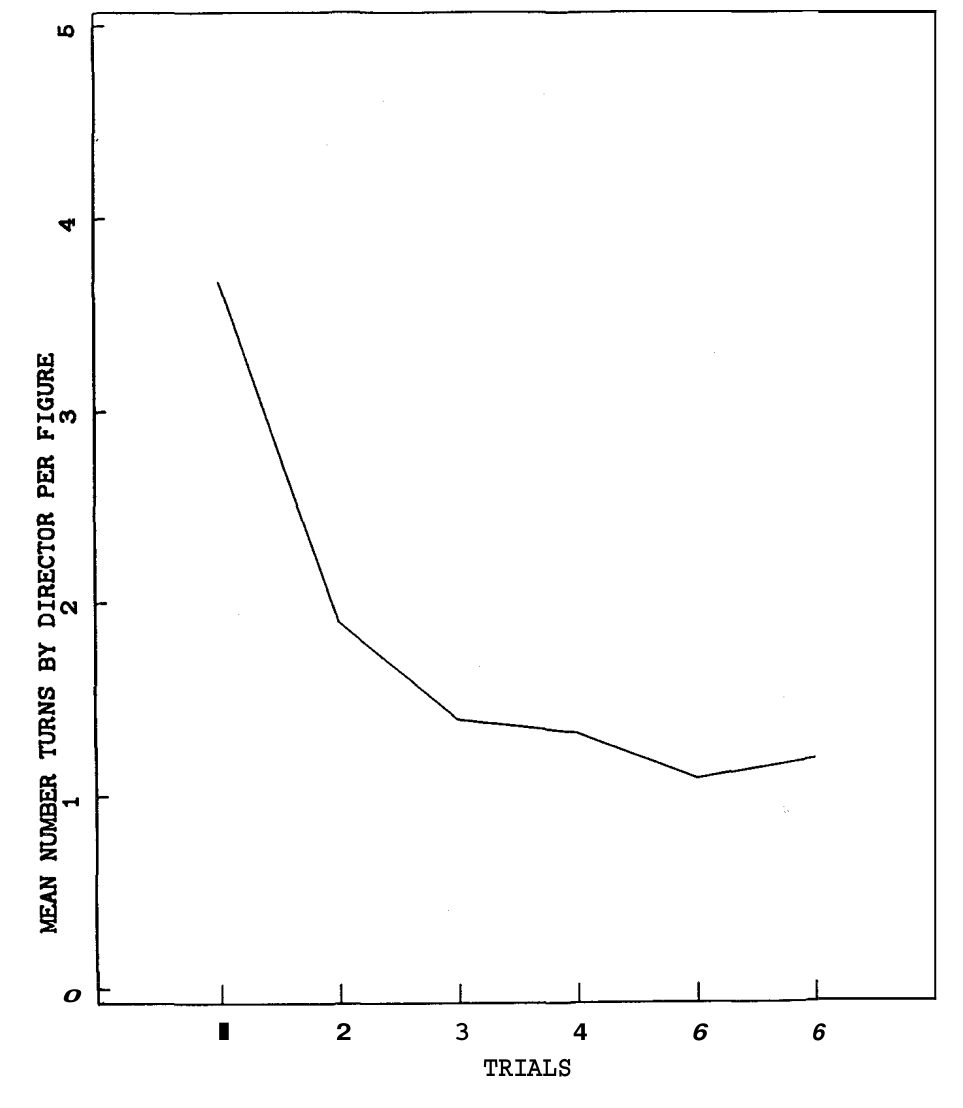
\includegraphics[width=.5\textwidth]{images/clark_turns.png}
\end{frame}
\begin{frame}{Yoon \& Brown-Schmidt 2019}
	Speaker talks to multiple matchers
	
			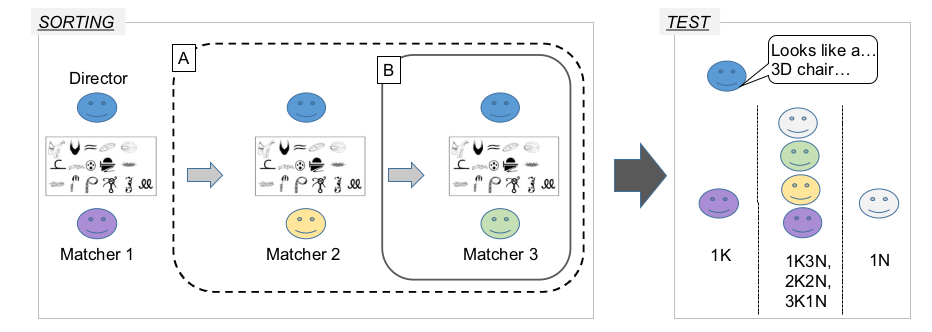
\includegraphics[width=\textwidth]{images/yoon_diagram.png}
			Speakers generally ``aim low'' 
\end{frame}
%
\begin{frame}{Hawkins, Frank, \& Goodman 2020}
Scaling up with web-based experiments
\begin{itemize}
	\item Cued version with feedback on each trial
	\item Message with a chat box
	\item After all exclusions, 83 dyads 
\end{itemize}
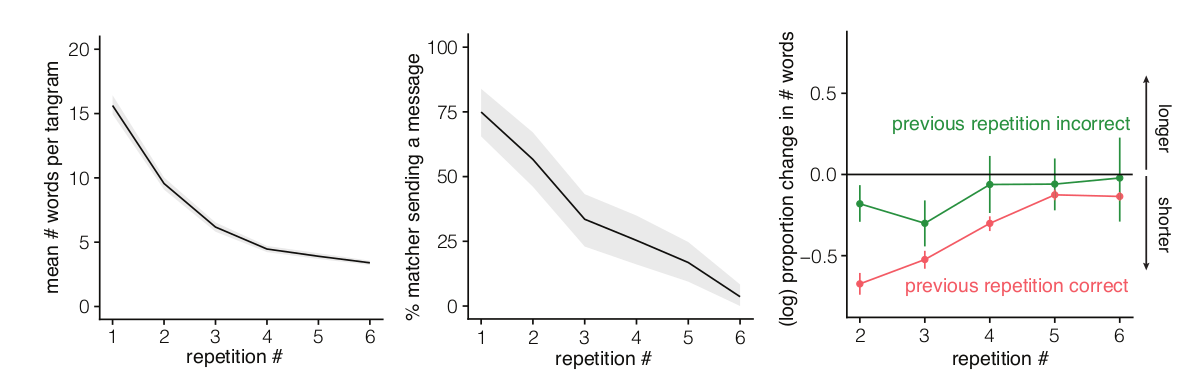
\includegraphics[width=\textwidth]{images/hawkins_fewer_words.png}
\end{frame}
%
\begin{frame}{Hawkins, Frank, \& Goodman 2020}
	NLP analytic techniques
	\begin{itemize}
		\item Syntactic -- words drop out as syntactic units
		\item Semantics -- more distinctive words conventionalize
	\end{itemize}
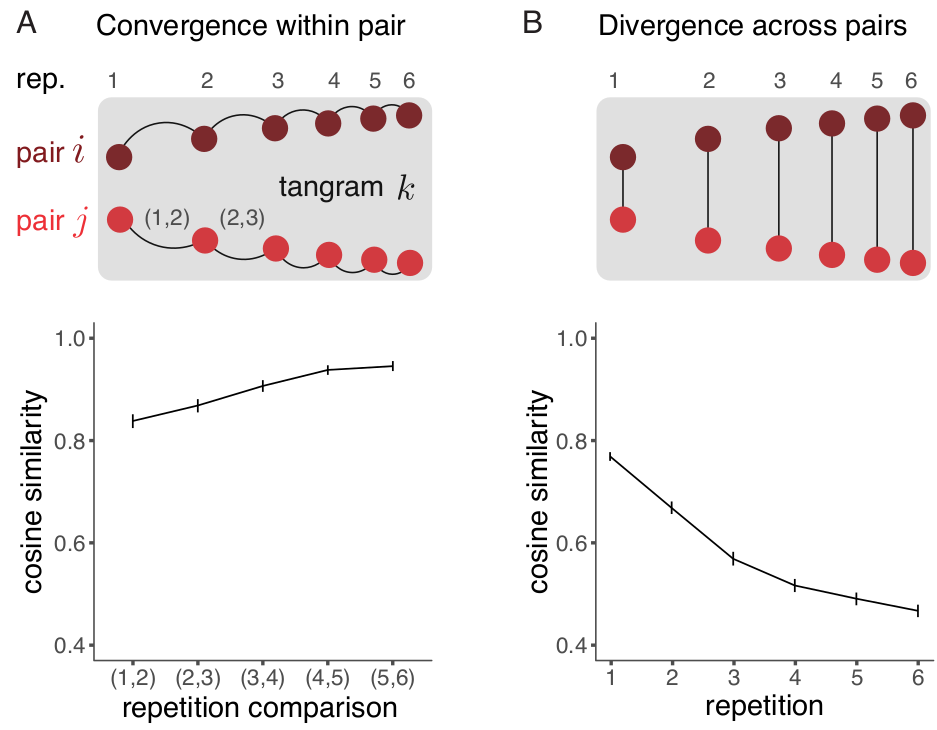
\includegraphics[width=.7\textwidth]{images/hawkins_converge.png}
\end{frame}
%
\begin{frame}{FYP Proposal}
	\begin{itemize}
		\item Replicate Hawkins et al for multiple listeners
		\item Bridges towards Yoon \& Brown-Schmidt work
		\item Use Empirica (Almaatouq et al 2020) for implementation
	\end{itemize}

\end{frame}

\begin{frame}{FYP Framework}

 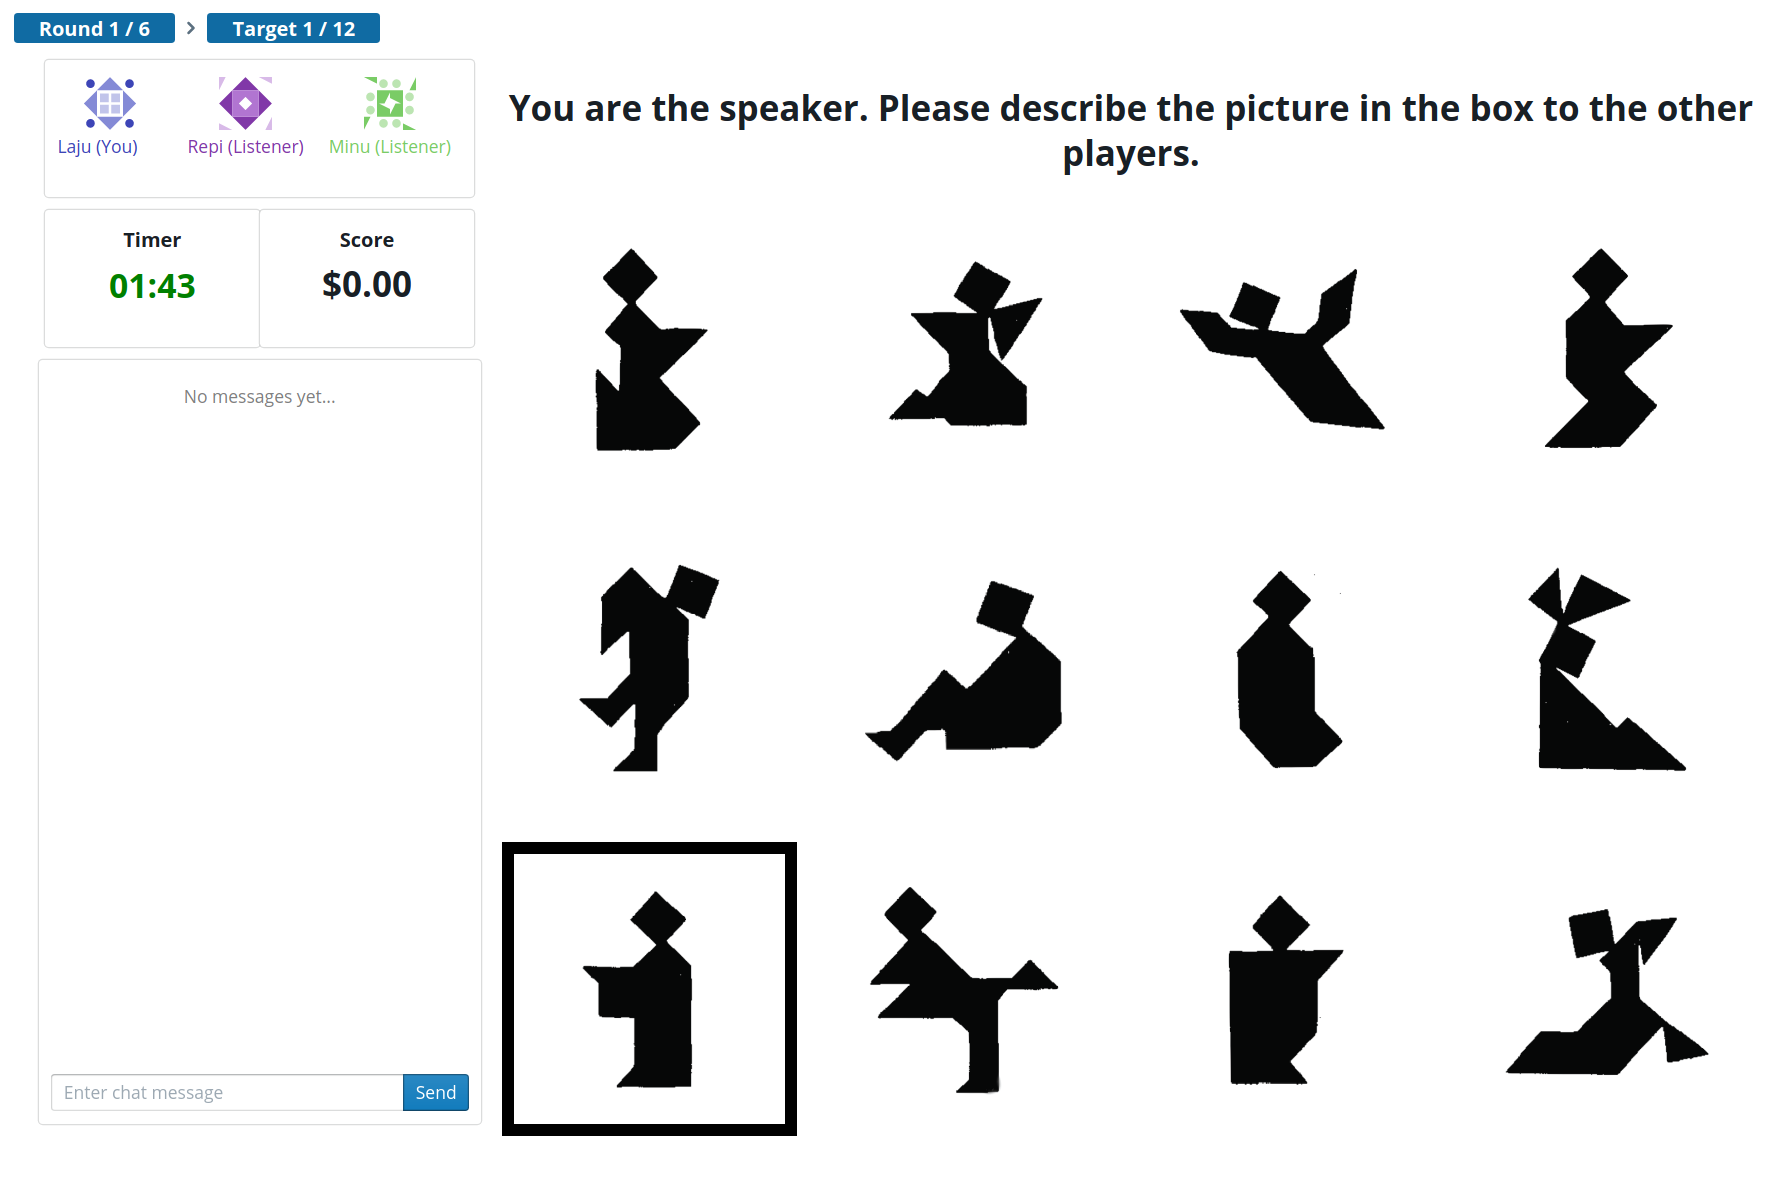
\includegraphics[width=.9\textwidth]{images/interface.PNG}
\end{frame}

\begin{frame}{Pilot results}
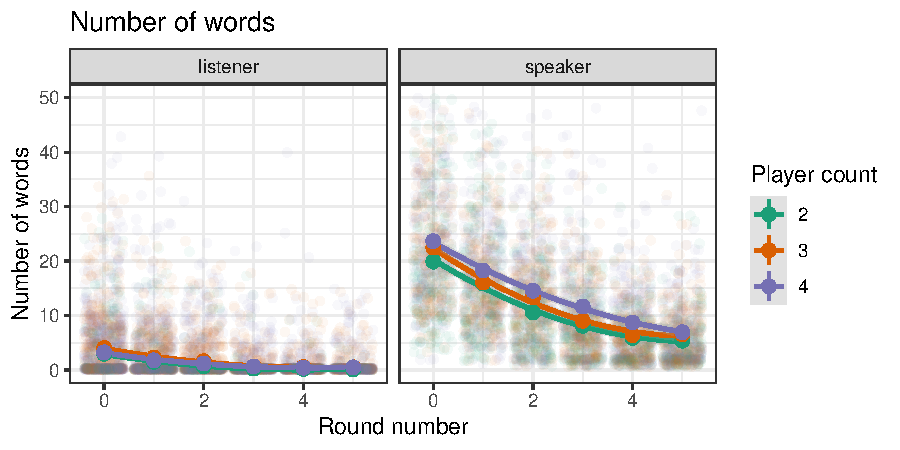
\includegraphics[width=\textwidth]{images/words.pdf}

\end{frame}

\begin{frame}{Pilot results}

	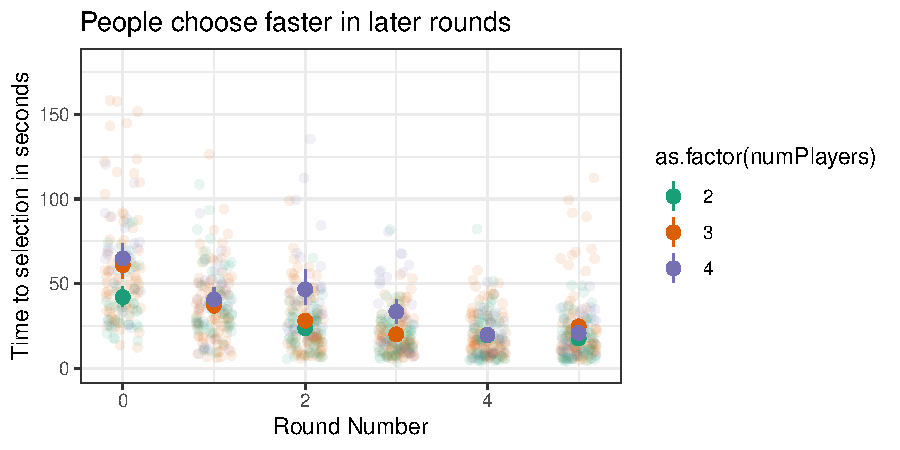
\includegraphics[width=\textwidth]{images/time.pdf}
	
\end{frame}

\begin{frame}{Pilot results}
	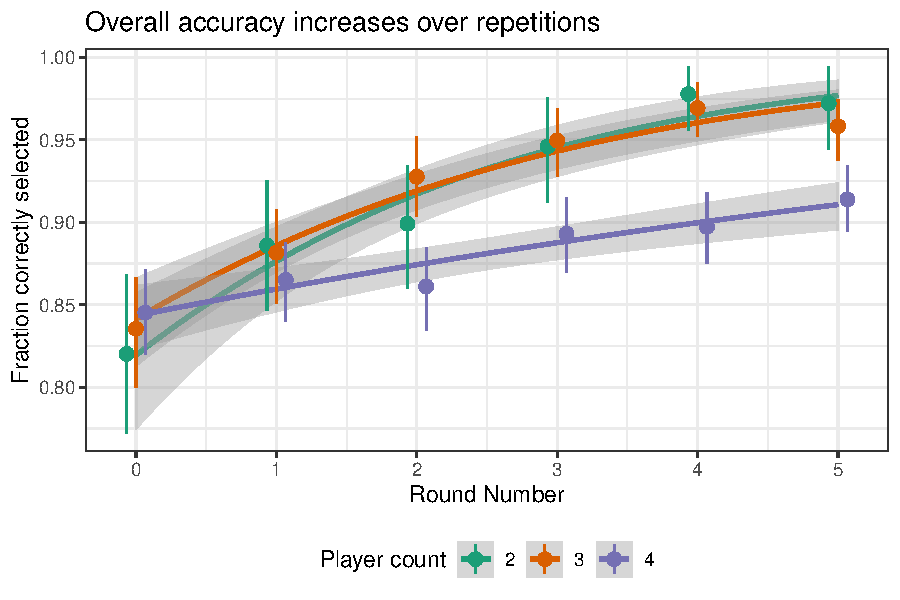
\includegraphics[width=\textwidth]{images/accuracy.pdf}
	
\end{frame}

\begin{frame}{FYP Plans}
	Future analyses
	\begin{itemize}
		\item Textual analyses
		\item Listener to listener interactions
		\item Test aim low hypothesis
	\end{itemize}

Full experiment
\begin{itemize}
	\item Test groups of 2-4 (1-3 listeners/speaker)
	\item Aim for 20 groups in each group size
\end{itemize}
\end{frame}

\begin{frame}{Other knobs}
	Very flexible framework
\begin{itemize}
	\item Number of players
	\item Target images
	\item Feedback and incentives 
	\item Rotating speaker role 
	\item Curriculum learning
\end{itemize}
\end{frame}

\end{document}

